\documentclass[aps,secnumarabic,amsmath,amssymb]{revtex4}
\usepackage{amsmath}
\usepackage{amssymb}
\usepackage{amsfonts}
\usepackage{color}
\usepackage{graphics}
\usepackage[pdftex]{graphicx}
\usepackage[utf8x]{inputenc}
\usepackage[colorlinks=true]{hyperref}
\usepackage{listings}

\newcommand{\ud}{\mathrm{d}}
\newcommand{\ue}{\mathrm{e}}
\newcommand{\ui}{\mathrm{i}}
\newcommand{\res}{\mathrm{Res}}
\newcommand{\Tr}{\mathrm{Tr}}
\newcommand{\dsum}{\displaystyle\sum}
\newcommand{\dprod}{\displaystyle\prod}
\newcommand{\dlim}{\dispqlaystyle\lim}
\newcommand{\dint}{\displaystyle\int}
\newcommand{\fsno}[1]{{\!\not\!{#1}}}
\newcommand{\texp}[2]{\ensuremath{{#1}\times10^{#2}}}
\newcommand{\dexp}[2]{\ensuremath{{#1}\cdot10^{#2}}}
\newcommand{\eval}[2]{{\left.{#1}\right|_{#2}}}
\newcommand{\paren}[1]{{\left({#1}\right)}}
\newcommand{\lparen}[1]{{\left({#1}\right.}}
\newcommand{\rparen}[1]{{\left.{#1}\right)}}
\newcommand{\abs}[1]{{\left|{#1}\right|}}
\newcommand{\sqr}[1]{{\left[{#1}\right]}}
\newcommand{\crly}[1]{{\left\{{#1}\right\}}}
\newcommand{\angl}[1]{{\left\langle{#1}\right\rangle}}
\newcommand{\tpdiff}[4][{}]{{\paren{\frac{\partial^{#1} {#2}}{\partial {#3}{}^{#1}}}_{#4}}}
\newcommand{\tpsdiff}[4][{}]{{\paren{\frac{\partial^{#1}}{\partial {#3}{}^{#1}}{#2}}_{#4}}}
\newcommand{\pdiff}[3][{}]{{\frac{\partial^{#1} {#2}}{\partial {#3}{}^{#1}}}}
\newcommand{\diff}[3][{}]{{\frac{\ud^{#1} {#2}}{\ud {#3}{}^{#1}}}}
\newcommand{\psdiff}[3][{}]{{\frac{\partial^{#1}}{\partial {#3}{}^{#1}} {#2}}}
\newcommand{\sdiff}[3][{}]{{\frac{\ud^{#1}}{\ud {#3}{}^{#1}} {#2}}}
\newcommand{\tpddiff}[4][{}]{{\left(\dfrac{\partial^{#1} {#2}}{\partial {#3}{}^{#1}}\right)_{#4}}}
\newcommand{\tpsddiff}[4][{}]{{\paren{\dfrac{\partial^{#1}}{\partial {#3}{}^{#1}}{#2}}_{#4}}}
\newcommand{\pddiff}[3][{}]{{\dfrac{\partial^{#1} {#2}}{\partial {#3}{}^{#1}}}}
\newcommand{\ddiff}[3][{}]{{\dfrac{\ud^{#1} {#2}}{\ud {#3}{}^{#1}}}}
\newcommand{\psddiff}[3][{}]{{\frac{\partial^{#1}}{\partial{}^{#1} {#3}} {#2}}}
\newcommand{\sddiff}[3][{}]{{\frac{\ud^{#1}}{\ud {#3}{}^{#1}} {#2}}}
\newcommand{\eff}{ef\! f}

\begin{document}
\title{Motional Ground-State Cooling Outside the Lamb-Dicke Regime -- Supplemental material}
\author{Y. Yu}
\email{yichaoyu@g.harvard.edu}
\author{N. R. Hutzler}
\altaffiliation{Present address: California Institute of Technology, Division of Physics, Mathematics, and Astronomy. Pasadena, CA, 91125}
\author{J. T. Zhang}
\author{L. R. Liu}
\author{T. Rosenband}
\author{K.-K. Ni}
\email{ni@chemistry.harvard.edu}
\affiliation{Department of Chemistry and Chemical Biology, Harvard University, Cambridge, Massachusetts, 02138, USA}
\affiliation{Department of Physics, Harvard University, Cambridge, Massachusetts, 02138, USA}
\affiliation{Harvard-MIT Center for Ultracold Atoms, Cambridge, Massachusetts, 02138, USA}

\date{\today}

\maketitle

\section{Raman Sideband Cooling Pulse Parameters and Sequence}
Here, we list the full Raman sideband cooling (RSC) pulse parameters and sequence used to obtain the result in the manuscript.
A step of RSC contains a Raman pulse and an optical pumping pulse.
The full RSC sequence includes 540 pulses in 53 ms.

\subsection{Optical pumping parameters}
The optical pumping is performed with a $\sigma^+$-polarized beam aligned with an 8.8 G bias magnetic field.
There are two frequencies in the beam: one is on resonance with
the $|F=2,m_F=1\rangle$ of $3^2S_{1/2}$ to $|F'=2,m_{F'}=2\rangle$ of $3^2P_{1/2}$ D1 transition
and the other is on resonance with the $|F=1,m_F=1\rangle$ of $3^2S_{1/2}$ to $|F'=2,m_{F'}=2\rangle$ of $3^2P_{3/2}$ D2 transition.
All optical pumping pulses have the length of $30\,\mu$s
with a scattering rate of $0.14$ MHz for atoms in $|F=1,m_F=1\rangle$
and a scattering rate of $0.39$ MHz for atoms in $|F=2,m_F=1\rangle$.

\subsection{Raman pulse parameters}
Each Raman pulse in the cooling sequence is followed immediately by an optical pumping pulse.
The full parameters for the Raman pulses, including the cooling ``axis'',
the sideband ``order ($\Delta n$)'', the cooling frequency ``$\delta '$",
the carrier ($\Delta n=0$) frequency ``$\delta_0'$'', the pulse ``duration'',
the pulse strength in ``$\Omega_0$'',
and the beam of which a non-uniform ``power ramp'' is applied, are listed in 6 groups below.
The applied cooling frequency, $\delta'$,
is the two-photon detuning given relative to the zero-field $F=1$ and $F=2$ hyperfine splitting
of $1.7716261288(10)$GHz~\cite{SteckNa}.
Due to the Stark shifts of the Raman beams, the carrier transition, $\delta'_0$,
varies with the power of the Raman beams.
$\delta'_0$ is given also relative to the zero-field hyperfine splitting.
The strength of the pulses given in $\Omega_0$ determines the two-photon Rabi frequency,
$\Omega_{n,\Delta n}=\Omega_0 \langle n|e^{i \vec{k} \cdot \vec{r}}|n+\Delta n\rangle$.
We adopt the convention that a $\pi$-pulse between state $n$ and $n+\Delta n$ requires a duration $\pi/\Omega_{n,\Delta n}$.
The difference between $\delta'$ and $\delta'_0$ gives the motional sideband frequency, $\delta$.
Many Raman pulses include a ``power ramp'' with a Blackman envelope~\cite{Kasevich1992} to minimize off-resonant excitations.
Because each Raman pulse is a product of two spatial- and temporal-overlapped laser beams,
the ``power ramp'' is applied only to the beam that has the smaller light shift
(we label the beam by the corresponding $F$ number) while the other beam has a square-pulse shape.
For a Raman pulse with a power ramp,
the Rabi frequency gives the arithmetic mean over the duration of the pulse.

\newpage

\subsubsection{Group 1}
This group is repeated 4 times.
\begin{center}
  \begin{tabular}{|c|c|c|c|c|c|c|}
    \hline
    Axis&$\Delta n$&$\delta'$ (MHz)&$\delta'_0$ (MHz)&Duration ($\mu$s)& $\Omega_0$ (kHz)&Power ramp\\\hline
    $x$&-2&$19.625$&$18.649$&44.1&$2\pi\times23$&F1\\\hline
    $y$&-2&$19.615$&$18.648$&28.6&$2\pi\times35$&F1\\\hline
    $x$&-1&$19.130$&$18.649$&36.9&$2\pi\times23$&F1\\\hline
    $y$&-1&$19.615$&$18.648$&24.0&$2\pi\times35$&F1\\\hline
  \end{tabular}
\end{center}

\subsubsection{Group 2}
This group is repeated 5 times.
\begin{center}
  \begin{tabular}{|c|c|c|c|c|c|c|}
    \hline
    Axis&$\Delta n$&$\delta'$ (MHz)&$\delta'_0$ (MHz)&Duration ($\mu$s)& $\Omega_0$ (kHz)&Power ramp\\\hline
    $z$&-5&$19.030$&$18.605$&81.5&$2\pi\times16$&F2\\\hline
    $x$&-2&$19.625$&$18.649$&44.1&$2\pi\times23$&F1\\\hline
    $z$&-4&$18.940$&$18.605$&76.3&$2\pi\times16$&F2\\\hline
    $y$&-2&$19.615$&$18.648$&28.6&$2\pi\times35$&F1\\\hline
    $z$&-5&$19.030$&$18.605$&81.5&$2\pi\times16$&F2\\\hline
    $x$&-1&$19.130$&$18.649$&36.9&$2\pi\times23$&F1\\\hline
    $z$&-4&$18.940$&$18.605$&76.3&$2\pi\times16$&F2\\\hline
    $y$&-1&$19.130$&$18.648$&24.0&$2\pi\times35$&F1\\\hline
  \end{tabular}
\end{center}
\subsubsection{Group 3}
This group is repeated 6 times.
\begin{center}
  \begin{tabular}{|c|c|c|c|c|c|c|}
    \hline
    Axis&$\Delta n$&$\delta'$ (MHz)&$\delta'_0$ (MHz)&Duration ($\mu$s)& $\Omega_0$ (kHz)&Power ramp\\\hline
    $z$&-4&$18.940$&$18.605$&76.3&$2\pi\times16$&F2\\\hline
    $x$&-2&$19.625$&$18.649$&44.1&$2\pi\times23$&F1\\\hline
    $z$&-3&$18.858$&$18.605$&70.2&$2\pi\times16$&F2\\\hline
    $y$&-2&$19.615$&$18.648$&28.6&$2\pi\times35$&F1\\\hline
    $z$&-4&$18.940$&$18.605$&76.3&$2\pi\times16$&F2\\\hline
    $x$&-1&$19.130$&$18.649$&36.9&$2\pi\times23$&F1\\\hline
    $z$&-3&$18.858$&$18.605$&70.2&$2\pi\times16$&F2\\\hline
    $y$&-1&$19.130$&$18.648$&24.0&$2\pi\times35$&F1\\\hline
  \end{tabular}
\end{center}

\newpage
\subsubsection{Group 4}
This group is repeated 7 times.
\begin{center}
  \begin{tabular}{|c|c|c|c|c|c|c|}
    \hline
    Axis&$\Delta n$&$\delta'$ (MHz)&$\delta'_0$ (MHz)&Duration ($\mu$s)& $\Omega_0$ (kHz)&Power ramp\\\hline
    $z$&-3&$18.858$&$18.605$&70.2&$2\pi\times16$&F2\\\hline
    $x$&-2&$19.625$&$18.649$&44.1&$2\pi\times23$&F1\\\hline
    $z$&-2&$18.773$&$18.605$&62.7&$2\pi\times16$&F2\\\hline
    $y$&-2&$19.615$&$18.648$&28.6&$2\pi\times35$&F1\\\hline
    $z$&-3&$18.858$&$18.605$&70.2&$2\pi\times16$&F2\\\hline
    $x$&-1&$19.130$&$18.649$&36.9&$2\pi\times23$&F1\\\hline
    $z$&-2&$18.773$&$18.605$&62.7&$2\pi\times16$&F2\\\hline
    $y$&-1&$19.130$&$18.648$&24.0&$2\pi\times35$&F1\\\hline
  \end{tabular}
\end{center}
\subsubsection{Group 5}
This group is repeated 10 times.
\begin{center}
  \begin{tabular}{|c|c|c|c|c|c|c|}
    \hline
    Axis&$\Delta n$&$\delta'$ (MHz)&$\delta'_0$ (MHz)&Duration ($\mu$s)& $\Omega_0$ (kHz)&Power ramp\\\hline
    $z$&-2&$18.773$&$18.605$&62.7&$2\pi\times16$&F2\\\hline
    $x$&-1&$19.130$&$18.649$&36.9&$2\pi\times23$&F1\\\hline
    $z$&-1&$18.685$&$18.605$&52.5&$2\pi\times16$&F2\\\hline
    $y$&-1&$19.130$&$18.648$&24.0&$2\pi\times35$&F1\\\hline
    $z$&-2&$18.773$&$18.605$&62.7&$2\pi\times16$&F2\\\hline
    $x$&-1&$19.130$&$18.649$&70.0&$2\pi\times23$&F1\\\hline
    $z$&-1&$18.685$&$18.605$&52.5&$2\pi\times16$&F2\\\hline
    $y$&-1&$19.130$&$18.648$&46.0&$2\pi\times35$&F1\\\hline
  \end{tabular}
\end{center}
\subsubsection{Group 6}
This group is repeated 30 times.
\begin{center}
  \begin{tabular}{|c|c|c|c|c|c|c|}
    \hline
    Axis&$\Delta n$&$\delta'$ (MHz)&$\delta'_0$ (MHz)&Duration ($\mu$s)& $\Omega_0$ (kHz)&Power ramp\\\hline
    $z$&-1&$18.683$&$18.605$&78.7&$2\pi\times11$&F2\\\hline
    $z$&-1&$18.683$&$18.605$&135.0&$2\pi\times11$&F2\\\hline
    $z$&-1&$18.685$&$18.605$&78.7&$2\pi\times11$&F2\\\hline
    $x$&-1&$19.130$&$18.649$&36.9&$2\pi\times23$&F1\\\hline
    $y$&-1&$19.130$&$18.648$&24.0&$2\pi\times35$&F1\\\hline
    $z$&-1&$18.685$&$18.605$&78.7&$2\pi\times11$&F2\\\hline
    $z$&-1&$18.685$&$18.605$&135.0&$2\pi\times11$&F2\\\hline
    $z$&-1&$18.685$&$18.605$&78.7&$2\pi\times11$&F2\\\hline
    $x$&-1&$19.130$&$18.649$&70.0&$2\pi\times23$&F1\\\hline
    $y$&-1&$19.130$&$18.648$&46.0&$2\pi\times35$&F1\\\hline
  \end{tabular}
\end{center}
\newpage

\section{Zoomed data for Raman Sideband Cooling}
Efficient RSC enables the preparation of single atoms with a high probability of being in the trap ground state.  That probability can be measured by Raman sideband spectroscopy.
Here we show a zoomed spectra after RSC for clarity.  The cooling orders ($\Delta n=-1,-2$ for radial x and y axes and $\Delta n=-1, \dots, -5$ for axial z axis) are shown.
Each data point comes from repeated measurements with more than 450 single atoms loaded.
The heights of these sidebands are about $2.5\%$. \\

\includegraphics[height=4cm]{spectrum_zoom_cool_rx.pdf}
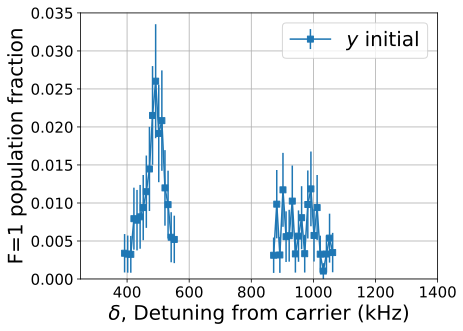
\includegraphics[height=4cm]{spectrum_zoom_cool_ry.pdf}
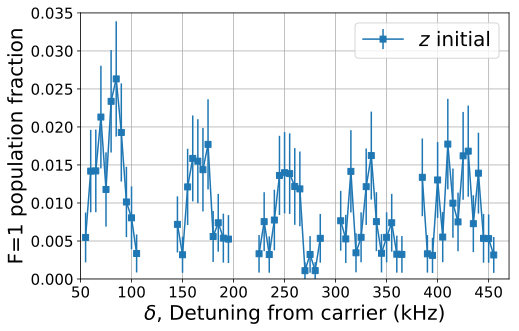
\includegraphics[height=4cm]{spectrum_zoom_cool_az.pdf}

\bibliography{paper}
\end{document}
